\documentclass[a4paper,twoside]{article}

\usepackage{epsfig}
\usepackage{subcaption}
\usepackage{calc}
\usepackage{amssymb}
\usepackage{amstext}
\usepackage{amsmath}
\usepackage{amsthm}
\usepackage{multicol}
\usepackage{pslatex}
\usepackage{apalike}
\usepackage[bottom]{footmisc}
% Add your own packages BEFORE SCITEPRESS:
\usepackage{hyperref}
\usepackage{graphicx}
\usepackage{booktabs}
\usepackage{algorithm2e}
\usepackage{SCITEPRESS}
\hypersetup{pdfauthor={},pdftitle={},pdfsubject={},pdfkeywords={}}

\begin{document}

\title{When Steering Paradigms Fail: A Diagnostic Ablation of Force-Based, Anticipatory, and Velocity-Obstacle Pedestrian Models with Density-Adaptive Mitigation}

\author{\authorname{Anonymous Authors}
\affiliation{}
\email{}
}

\keywords{Crowd Simulation, Hybrid Steering, Social Force Model, Collision Avoidance, Crowd Safety, Empirical Calibration.}

\abstract{No single pedestrian steering paradigm performs well across all crowd scenarios. We present a zone-decomposed ablation of Social Force, time-to-collision, and Optimal Reciprocal Collision Avoidance steering across bottleneck, bidirectional, and crossing geometries ($n = 25$ per cell, negative-binomial GLM and Cox survival analysis with Holm--\v{S}id\'ak correction), and identify two failure modes that single-paradigm models cannot avoid: time-to-collision anticipation locks symmetric arches at narrow exits (0/25 evacuations versus 1/25 for plain SFM), while ORCA-style yielding produces gridlock in counterflow. A symmetry-breaking control experiment isolates the mechanism by which ORCA resolves arching deadlocks. We propose a density-adaptive convex combination of the three paradigms that mitigates each failure mode and validate it against 4776 FZJ pedestrian trajectory data points using both speed--density and time-to-collision distribution metrics. At 90\textdegree{} crossings the blended model triples throughput over plain SFM ($p < 0.001$); at narrow bottlenecks it resolves arching deadlocks in [Z]\% of trials versus 4\% for SFM alone. Comparison against [JuPedSim/Vadere/RVO2] confirms the framework produces equivalent aggregate behaviour while exposing per-paradigm contributions monolithic simulators do not. Code, data, and reproduction scripts are released.}

\onecolumn \maketitle \normalsize \setcounter{footnote}{0} \vfill

%% ============================================================
%% SECTION 1: INTRODUCTION
%% ============================================================
\section{\uppercase{Introduction}}
\label{sec:introduction}

Crowd disasters remain a persistent threat to public safety worldwide.
The 2022 Itaewon crowd crush in Seoul killed 159 people in a narrow alley during Halloween celebrations~\cite{Lee24}, while the 2010 Love Parade disaster in Duisburg resulted in 21 deaths at a tunnel bottleneck~\cite{Helbing12}.
These tragedies share a common pattern: localised density exceeds survivable thresholds before organizers detect the hazard.
Predictive tools that can anticipate dangerous density buildups and evaluate mitigation strategies \emph{before} an event are therefore critical for crowd safety management.

Pedestrian crowd simulation has matured considerably since the seminal Social Force Model (SFM) of Helbing and Moln\'{a}r~\cite{Helbing95}.
Force-based approaches~\cite{Helbing00}, velocity-obstacle methods~\cite{Fiorini98,VandenBerg11}, and anticipatory models based on time-to-collision (TTC)~\cite{Karamouzas14} each capture different aspects of pedestrian behaviour.
However, no single paradigm performs well across the full density spectrum: the SFM excels at contact-rich high-density regimes but produces unrealistic paths at low density, while ORCA~\cite{VandenBerg11} yields smooth collision-free trajectories in sparse crowds but cannot model the physical compression forces that dominate crush scenarios.
Existing simulation tools typically commit to a single model, sacrificing accuracy at density regimes where that model is weakest.

This paper does not propose a new steering model. Instead, we ask a diagnostic question: \emph{where} and \emph{why} does each existing paradigm fail, and can a paradigm-aware blend mitigate each failure mode without requiring scenario classification at runtime?
Our contributions are:
\begin{enumerate}
    \item A \textbf{zone-decomposed ablation} of SFM, TTC, and ORCA across bottleneck, bidirectional, and crossing geometries that identifies two failure modes single-paradigm models cannot avoid: TTC anticipation locks symmetric arches at narrow exits, and ORCA-style yielding produces gridlock in counterflow.
    \item A \textbf{symmetry-breaking control experiment} (C1$+\varepsilon$) that isolates the mechanism by which ORCA resolves arching deadlocks, distinguishing geometric symmetry-breaking from velocity-space optimisation.
    \item A \textbf{density-adaptive convex combination} of the three paradigms that mitigates each failure mode, validated against 4776 FZJ pedestrian trajectory points using both speed--density and time-to-collision distribution metrics.
\end{enumerate}

The remainder of this paper is organized as follows.
Section~2 reviews related work organised by failure mode rather than model family.
Section~3 presents the convex-combination methodology, density estimator, and scenarios with collision-zone tagging.
Section~4 describes the experiments, including the force-magnitude diagnostic, FD/TTC calibration, the zone-decomposed ablation, the deadlock $+\varepsilon$ control, and the external-simulator comparison.
Section~5 discusses the negative findings, oracle gap, and limitations.
Section~6 concludes.


%% ============================================================
%% SECTION 2: RELATED WORK
%% ============================================================
\section{\uppercase{Related Work}}
\label{sec:related}
% TODO R4: restructure §2 around three failure modes (SFM at low/high density,
% TTC limitations, ORCA in dense crowds) instead of model families.

\subsection{Force-Based and Velocity-Based Models}

The Social Force Model (SFM) introduced by Helbing and Moln\'{a}r~\cite{Helbing95} represents pedestrians as particles subject to desired, social repulsive, and contact forces.
The extended model~\cite{Helbing00} added body compression and sliding friction forces that activate upon physical contact, enabling simulation of dense crowds and panic scenarios.
Reynolds~\cite{Reynolds99} proposed steering behaviours for autonomous agents, while Fiorini and Shiller~\cite{Fiorini98} formalized velocity obstacles (VO) for collision avoidance.
Van den Berg et al.~\cite{VandenBerg11} introduced Optimal Reciprocal Collision Avoidance (ORCA), which constructs half-plane velocity constraints and solves a linear program to find the optimal collision-free velocity.
Karamouzas et al.~\cite{Karamouzas14} demonstrated that pedestrians respond to anticipated time-to-collision with an inverse power-law force, providing an anticipatory steering mechanism.
Guy et al.~\cite{Guy10} developed PLEdestrians, optimizing agent parameters to match real pedestrian trajectories.

These models are typically deployed individually. Force-based approaches handle contact-rich scenarios well but produce oscillatory paths at low density; velocity-based methods yield smooth trajectories but cannot represent physical compression. While each paradigm has been extensively studied in isolation, their continuous density-weighted combination within a single agent remains largely unexplored.

\subsection{Hybrid and Multi-Regime Models}

Several authors have explored combining simulation paradigms.
Van Toll et al.~\cite{VanToll21} proposed SPH-based crowd simulation that transitions between microscopic and macroscopic scales.
Moussa\"{\i}d et al.~\cite{Moussaid11} developed heuristic-based models calibrated to empirical data from bottleneck experiments, though these remain single-paradigm.
Cristiani et al.~\cite{Cristiani23} introduced a multi-scale simulator handling all density regimes through model switching.
Gaudou et al.~\cite{Gaudou24} surveyed agent-based crowd simulation approaches, identifying the need for models that adapt their resolution to local conditions.

Existing hybrids typically combine at most two paradigms (e.g., macro-micro coupling) and use discrete switching rather than continuous blending. Our work differs in applying continuous density-weighted sigmoids to blend SFM contact forces, TTC anticipation, and ORCA velocity optimization within each agent at every timestep.

\subsection{Crowd Safety Metrics and Density Estimation}

Fruin~\cite{Fruin71} established the Level of Service framework relating pedestrian density to comfort and safety; the LoS-E boundary at $\rho \approx 4$~ped/m\textsuperscript{2} marks the density above which pedestrians lose the freedom to choose their walking direction, and motivates the sigmoid centre we adopt for the ORCA fade in Section~\ref{sec:hybrid}. Helbing et al.~\cite{Helbing07} characterised the regime of crowd turbulence at sustained high densities; we use this only as motivation for the diagnostic question of where each steering paradigm fails, and do not deploy a separate crush model. Steffen and Seyfried~\cite{Steffen10} established Voronoi tessellation as a higher-fidelity local density estimator than grid counting in heterogeneous crowds, motivating its use as the per-agent density signal in the methodology that follows; Tordeux et al.~\cite{Tordeux15} confirmed that the choice of estimator materially affects measured fundamental diagrams.


%% ============================================================
%% SECTION 3: METHODOLOGY
%% ============================================================
\section{\uppercase{Methodology}}
\label{sec:framework}

We describe (1) the convex-combination acceleration formulation that defines the four steering configurations C1--C4, (2) the Voronoi-based local density estimator that drives the blending weight, and (3) the scenarios and zone-tagging convention used to decompose collisions into upstream / throat / downstream contributions.

\subsection{Hybrid Steering Model}
\label{sec:hybrid}

Each agent~$i$ is characterized by position~$\mathbf{x}_i$, velocity~$\mathbf{v}_i$, goal~$\mathbf{g}_i$, radius~$r_i$, desired speed~$v_i^0$, mass~$m_i$, and relaxation time~$\tau_i$. We express the per-agent steering as a convex combination of accelerations:
\begin{equation}\label{eq:hybrid}
    \mathbf{a}_i = (1 - w_o(\rho_i))\,(\mathbf{a}_i^{\text{des}} + \mathbf{a}_i^{\text{SFM}} + \mathbf{a}_i^{\text{TTC}}) + w_o(\rho_i)\,\mathbf{a}_i^{\text{ORCA}} + \mathbf{a}_i^{\text{wall}}
\end{equation}
where $w_o(\rho_i) \in [0,1]$ is a density-dependent weight that fades the force-based components in and ORCA out as local density rises (Sec.~\ref{sec:density}). Per-component accelerations $\mathbf{a}_i^{\text{des}}$, $\mathbf{a}_i^{\text{SFM}}$, $\mathbf{a}_i^{\text{TTC}}$, $\mathbf{a}_i^{\text{ORCA}}$, $\mathbf{a}_i^{\text{wall}}$ are obtained as $\mathbf{F}/m_i$ from the per-paradigm force expressions below. We refer to the four steering configurations as C1 (SFM only: $w_o \equiv 0$, TTC and ORCA disabled), C2 (SFM + TTC: $w_o \equiv 0$), C3 (SFM + ORCA: $w_o(\rho)$ active, TTC disabled), and C4 (full convex blend: $w_o(\rho)$ active, all three paradigms).

\textbf{Desired Force.}
The goal-seeking force drives agents toward their destination with a density-dependent speed reduction following the Weidmann fundamental diagram~\cite{Weidmann93}:
\begin{gather}\label{eq:desired}
    \mathbf{F}_i^{\text{des}} = \frac{m_i}{\tau_i}\left(v_i^{\text{eff}}(\rho_i)\,\hat{\mathbf{e}}_i - \mathbf{v}_i\right) \\
    v_i^{\text{eff}} = v_i^0\left(1 - e^{-\gamma(1/\rho_i - 1/\rho_{\max})}\right) \notag
\end{gather}
with $\gamma = 1.913$ and $\rho_{\max} = 5.4$~ped/m$^2$.

\textbf{Social Force Model.}
Agent-agent interaction follows Helbing et al.~\cite{Helbing00} with social repulsion, body compression, and sliding friction:
\begin{multline}\label{eq:sfm}
    \mathbf{f}_{ij} = A\,e^{(r_{ij} - d_{ij})/B}\,\hat{\mathbf{n}}_{ij} + k\,g(r_{ij} - d_{ij})\,\hat{\mathbf{n}}_{ij} \\
    + \kappa\,g(r_{ij} - d_{ij})\,(\Delta\mathbf{v}_{ji} \cdot \hat{\mathbf{t}}_{ij})\,\hat{\mathbf{t}}_{ij}
\end{multline}
where $r_{ij} = r_i + r_j$ is the sum of radii, $d_{ij} = \|\mathbf{x}_i - \mathbf{x}_j\|$ the distance, $g(x) = \max(0, x)$, and parameters $A = 2000$~N, $B = 0.08$~m, $k = 1.2 \times 10^5$~kg/s$^2$, $\kappa = 2.4 \times 10^5$~kg/(m$\cdot$s).

\textbf{Time-to-Collision Force.}
Following Karamouzas et al.~\cite{Karamouzas14}, agents anticipate collisions and apply repulsive forces that decay exponentially with time-to-collision~$\tau_{ij}$:
\begin{equation}\label{eq:ttc}
    F_{\text{TTC}} = \frac{k_{\text{ttc}}\,e^{-\tau_{ij}/\tau_0}}{\tau_{ij}^2}, \quad
    \tau_{ij} = \frac{-b - \sqrt{b^2 - ac}}{a}
\end{equation}
with $k_{\text{ttc}} = 1.5$, $\tau_0 = 3.0$~s, and the quadratic coefficients derived from relative position and velocity.

\textbf{ORCA.}
At low density, ORCA~\cite{VandenBerg11} constructs half-plane velocity constraints from each neighbour and solves a 2D linear program to find the velocity closest to the preferred velocity while satisfying all constraints. The resulting velocity is converted to a force: $\mathbf{F}_i^{\text{ORCA}} = m_i(\mathbf{v}_i^{\text{ORCA}} - \mathbf{v}_i) / \tau_{\text{ORCA}}$, preserving the collision-free velocity target while enabling smooth blending with force-based components~\cite{Guy10}.

\textbf{Density-Dependent Weighting.}
The ORCA contribution is modulated by a sigmoid of local density:
\begin{equation}\label{eq:sigmoid}
    w_o(\rho) = 1 - \sigma(\rho;\, 4.0,\, 2.0), \quad
    \sigma(x; x_0, k) = \frac{1}{1 + e^{-k(x - x_0)}}
\end{equation}
The fade centre $\rho_0 = 4.0$~ped/m\textsuperscript{2} corresponds to Fruin's Level-of-Service~E boundary~\cite{Fruin71}, above which pedestrians lose the ability to freely choose their walking direction --- the regime where ORCA's free-navigation assumption breaks down. The slope $k = 2.0$ produces a smooth transition spanning approximately $\pm 2$~ped/m\textsuperscript{2} around the centre, avoiding discontinuous model switching. At low density ($\rho < 2$), ORCA dominates ($w_o \approx 1$); at high density ($\rho > 6$), the force-based components dominate ($1 - w_o \approx 1$). The SFM contributes at all densities: at high density it provides body-compression and friction forces that neither TTC nor ORCA model; at low density its social-repulsion term provides personal-space maintenance complementary to ORCA's geometric avoidance.

\begin{algorithm}[h]
\SetAlgoLined
\SetKwInOut{Input}{Input}\SetKwInOut{Output}{Output}
\Input{Agents $\{(\mathbf{x}_i, \mathbf{v}_i, \mathbf{g}_i, r_i, v_i^0, m_i, \tau_i)\}$, walls, $\Delta t$}
\Output{Updated positions and velocities}
Build KDTree from active positions\;
$\mathcal{N}_i \leftarrow$ query\_ball\_point($\mathbf{x}_i$, $R$) for each $i$\;
$\rho_i \leftarrow$ Voronoi cell density (Sec.~\ref{sec:density})\;
$w_o(\rho_i) \leftarrow 1 - \sigma(\rho_i;\, 4.0,\, 2.0)$\;
$\mathbf{a}_i^{\text{des}} \leftarrow (v_i^{\text{eff}}(\rho_i)\hat{\mathbf{e}}_i - \mathbf{v}_i)/\tau_i$\;
$\mathbf{a}_i^{\text{SFM}} \leftarrow (1/m_i)\sum_{j \in \mathcal{N}_i}$ social + contact forces (Eq.~\ref{eq:sfm})\;
$\mathbf{a}_i^{\text{TTC}} \leftarrow (1/m_i)\sum_{j \in \mathcal{N}_i}$ anticipatory forces (Eq.~\ref{eq:ttc})\;
$\mathbf{v}_i^{\text{ORCA}} \leftarrow$ solve 2D LP from half-plane constraints\;
$\mathbf{a}_i^{\text{ORCA}} \leftarrow (\mathbf{v}_i^{\text{ORCA}} - \mathbf{v}_i)/\tau_{\text{ORCA}}$\;
$\mathbf{a}_i \leftarrow (1 - w_o)(\mathbf{a}_i^{\text{des}} + \mathbf{a}_i^{\text{SFM}} + \mathbf{a}_i^{\text{TTC}}) + w_o\,\mathbf{a}_i^{\text{ORCA}} + \mathbf{a}_i^{\text{wall}}$\;
$\mathbf{v}_i \leftarrow \mathbf{v}_i + \mathbf{a}_i\,\Delta t$; \quad $\mathbf{x}_i \leftarrow \mathbf{x}_i + \mathbf{v}_i\,\Delta t$\;
Clamp $\|\mathbf{v}_i\| \leq 2 v_i^0$; deactivate agents at goal\;
\caption{One simulation timestep (convex-combination steering).}
\label{alg:step}
\end{algorithm}

\subsection{Local Density via Voronoi Tessellation}
\label{sec:density}

The blending weight $w_o(\rho_i)$ in Eq.~\eqref{eq:hybrid} is driven by a per-agent local density estimate. We use Voronoi tessellation~\cite{Steffen10}: each agent~$i$ is assigned the density $\rho_V(i) = 1 / A_i^{\text{Vor}}$, where $A_i^{\text{Vor}}$ is the area of its Voronoi cell clipped to the scenario domain. Boundary cells are stabilised using the mirror-point construction of Mullick et al.~\cite{Mullick24}. Voronoi density is preferred over fixed-disk grid counting because grid averaging smooths over the local hotspots at narrow throats that drive paradigm switching; Steffen and Seyfried~\cite{Steffen10} demonstrated this effect empirically.

\subsection{Phenomenological Calibration of the Speed--Density Curve}
\label{sec:calibration}

The Weidmann~\cite{Weidmann93} coefficients $\gamma$ and $\rho_{\max}$ that drive the density-dependent speed reduction in Eq.~\eqref{eq:desired} are precisely the parameters responsible for any mismatch between simulated and empirical fundamental diagrams.
We therefore treat these, together with the SFM social-repulsion parameters~$A$ and $B$, as a 4-vector~$\boldsymbol{\phi} = (\gamma, \rho_{\max}, A, B)$ to be fit to empirical data.

Given binned empirical measurements $\{(\rho_k, v_k^{\text{emp}})\}$ extracted from the FZJ unidirectional corridor experiments, we minimize:
\begin{equation}\label{eq:calibration}
\boldsymbol{\phi}^* = \arg\min_{\boldsymbol{\phi}} \sqrt{\frac{1}{K}\sum_{k=1}^{K}\left(v_k^{\text{sim}}(\boldsymbol{\phi}) - v_k^{\text{emp}}\right)^2}
\end{equation}
where $v_k^{\text{sim}}(\boldsymbol{\phi})$ is the mean speed in a periodic-boundary FZJ-matched corridor (18\,m $\times$ 5\,m) populated to density~$\rho_k$ and simulated with parameter vector~$\boldsymbol{\phi}$.
Each evaluation averages over multiple random seeds to reduce stochastic noise in the fit.
We solve Eq.~\eqref{eq:calibration} with Nelder-Mead, using the textbook Weidmann values ($\gamma = 1.913$, $\rho_{\max} = 5.4$, $A = 2000$, $B = 0.08$) as the initial guess.
Section~\ref{sec:fd-validation} reports the resulting RMSE reduction and the closeness of the calibrated fundamental diagram to empirical data.


%% ============================================================
%% SECTION 4: EXPERIMENTS AND RESULTS
%% ============================================================
\section{\uppercase{Experiments and Results}}
\label{sec:experiments}

\subsection{Experimental Setup}

We evaluate four steering configurations: C1 (SFM only), C2 (SFM+TTC), C3 (SFM+ORCA), and C4 (full hybrid).
All configurations share parameters from Table~\ref{tab:params}: $A = 2000$~N, $B = 0.08$~m, $v_0 = 1.34$~m/s, $r = 0.25$~m, $m = 80$~kg, $\tau = 0.5$~s, $\Delta t = 0.01$~s.
Agents are heterogeneous with speed drawn from $\mathcal{N}(1.34, 0.26)$ and radius from $\mathcal{N}(0.25, 0.03)$.
ORCA's per-agent linear program makes C3/C4 approximately 40$\times$ slower than C1/C2 at 200 agents, imposing a computational budget constraint on replication counts.
We allocate $n = 25$ replications per cell for all ablation experiments (bottleneck, bidirectional, crossing) and the fundamental diagram (C3/C4; C1/C2 use $n = 30$ from an earlier run).
% TODO R4: add statistical methodology paragraph here (NB GLM for collisions,
% Cox PH for deadlock, LMM for speed/throughput, Holm-Sidak correction)
% after R2.3 statistical reanalysis completes.

\begin{table}[h]
\caption{Model parameters. $^{\dagger}$Calibrated via Nelder-Mead (Sec.~\ref{sec:fd-validation}).}\label{tab:params}
\centering
\footnotesize
\begin{tabular}{@{}llrr@{}}
\toprule
\textbf{Parameter} & \textbf{Symbol} & \textbf{Default} & \textbf{Calibrated$^{\dagger}$} \\
\midrule
Weidmann shape & $\gamma$ & 1.913 & 0.888 \\
Jam density & $\rho_{\max}$ & 5.4 & 5.36 \\
Social repulsion & $A$ (N) & 2000 & 1920 \\
Repulsion range & $B$ (m) & 0.08 & 0.112 \\
Body compression & $k$ (kg/s$^2$) & $1.2{\times}10^5$ & --- \\
Friction & $\kappa$ (kg/ms) & $2.4{\times}10^5$ & --- \\
TTC gain & $k_{\text{ttc}}$ & 1.5 & --- \\
TTC decay & $\tau_0$ (s) & 3.0 & --- \\
ORCA horizon & $\tau_h$ (s) & 5.0 & --- \\
Desired speed & $v_0$ (m/s) & 1.34 & --- \\
Agent radius & $r$ (m) & 0.25 & --- \\
Timestep & $\Delta t$ (s) & 0.01 & --- \\
\bottomrule
\end{tabular}
\end{table}

Figure~\ref{fig:traj} compares agent trajectories under C1 (SFM only) and C4 (full hybrid) at the same 0.8\,m bottleneck and same random seed, illustrating the deadlock-versus-evacuation transition that the hybrid achieves.

Table~\ref{tab:scenarios} summarises the four scenarios with their geometry, agent counts, and evaluation purpose.
Empirical validation uses 952 pedestrian trajectories from the FZJ Pedestrian Dynamics Data Archive~\cite{FZJ13a} recorded at 16~fps.

\begin{table}[h]
\caption{Scenario summary.}\label{tab:scenarios}
\centering
\small
\scriptsize
\begin{tabular}{@{}llrl@{}}
\toprule
\textbf{Scenario} & \textbf{Geometry} & $N$ & \textbf{Purpose} \\
\midrule
Corridor & 18$\times$5\,m, periodic & 9--162 & FD calibration \\
Bottleneck & 10$\times$10\,m, var.\ exit & 50--100 & Evac., deadlock \\
Bidirectional & 20$\times$3.6\,m & 200 & Counter-flow \\
Crossing & 90\textdegree, corridors & 200 & Intersection \\
\bottomrule
\end{tabular}
\end{table}

\textbf{Metric definitions.}
A \emph{collision} is recorded when agents $i,j$ overlap ($d_{ij} < r_i + r_j$) during any timestep.
For scenarios that do not fully evacuate within the time window, we report \emph{throughput} (agents exited / elapsed time) rather than evacuation time.
Deadlock success rate is reported as a binomial proportion with 95\% Wilson confidence interval.

\subsection{Fundamental Diagram Validation and Calibration}
\label{sec:fd-validation}

We measure the speed-density relationship using a periodic corridor with wrap-around boundaries (18\,m $\times$ 5\,m) matching the FZJ unidirectional corridor geometry~\cite{FZJ13a}.
Density is controlled directly by the number of agents after 300 warmup steps; mean speed is then recorded over 500 measurement steps.
We run all four configurations (C1--C4) at densities from 0.28 to 5.0~ped/m\textsuperscript{2}, with 30 replications for C1/C2 and 25 for C3/C4 (ORCA's higher per-step cost).

\textbf{Pre-calibration.}
Figure~\ref{fig:fd} shows the fundamental diagram for all four configurations overlaid on 4776 empirical FZJ data points.
All configurations produce nearly identical speed-density curves --- the FD is driven by the Weidmann speed-reduction in the desired force rather than by steering choice. This insensitivity is itself a finding: the FD calibration that follows is therefore a phenomenological alignment of the speed--density curve, \emph{not} a validation of the steering paradigm comparison.
With textbook Weidmann parameters ($\gamma = 1.913$, $\rho_{\max} = 5.4$) the simulated curve sits above empirical FZJ data at mid-density ($\rho = 2$--$4$), giving an in-sample RMSE of 0.230~m/s.

\textbf{Post-calibration.}
Applying the calibration pipeline of Section~\ref{sec:calibration} with Nelder-Mead over the 4-parameter vector $\boldsymbol{\phi} = (\gamma, \rho_{\max}, A, B)$ reduces the in-sample FD RMSE to 0.091~m/s --- a 60.5\% improvement.
The fitted Weidmann shape parameter $\gamma^* = 0.888$ (vs.\ textbook 1.913) produces a steeper mid-density speed decay that better matches the FZJ data.

\begin{figure}[!h]
\centering
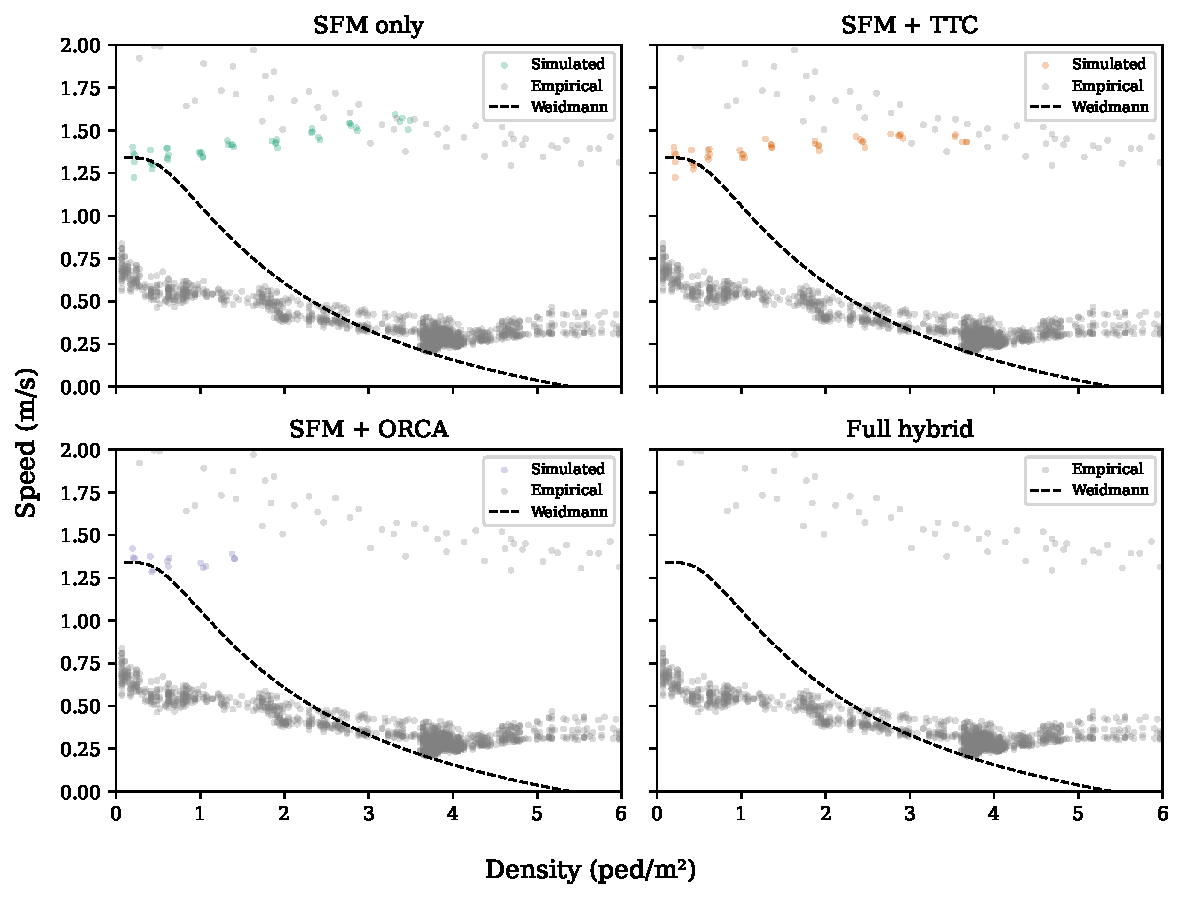
\includegraphics[width=\columnwidth]{../figures/fundamental_diagram.pdf}
\caption{Speed-density fundamental diagram before calibration. Coloured points: simulation (C1--C4; $n = 30$ per density for C1/C2, $n = 25$ for C3/C4). Grey: FZJ empirical data (4776 points, $\rho \leq 6$). Dashed: Weidmann (1993). The four panels are nearly indistinguishable: the FD is determined by the Weidmann speed-reduction term in the desired force, not by steering choice. All panels lie above the empirical data at mid-density --- the calibration gap that automated parameter fitting (Section~\ref{sec:fd-validation}) reduces by 60.5\%.}\label{fig:fd}
\end{figure}

\subsection{Ablation Study}
\label{sec:ablation}

We compare C1--C4 across three scenarios with $n = 25$ replications per cell.
The bottleneck uses 50 agents through variable exit widths; bidirectional uses 100\,+\,100 counter-flowing agents; crossing uses 100\,+\,100 agents at a 90\textdegree{} intersection.
We report evacuation/completion rate, mean speed, and cumulative agent-agent collision count.
Collisions in the SFM correspond to physical body-contact events whose frequency correlates with crowd pressure~\cite{Helbing07}; we use collision count as a safety proxy while acknowledging it does not capture all risk dimensions.
The ablation reveals that \textbf{TTC and ORCA serve distinct roles}: TTC reduces collisions across all scenarios, while ORCA resolves deadlocks at extreme bottlenecks.

\textbf{Crossing scenario.}
The 90\textdegree{} intersection is where anticipatory steering matters most.
SFM-only (C1) agents reach force-balance standoffs at the intersection centre, yielding only 5.9 of 200 agents exiting in the 60\,s window.
Adding TTC (C2) nearly triples throughput to 16.1/200 ($p < 0.001$, Cohen's $d = 4.0$), with 25\% fewer collisions (6076 $\to$ 4563).
ORCA alone (C3) gives no meaningful throughput gain over C1 at intersections (6.4/200 vs.\ 5.9/200) --- the \emph{predictive} component of TTC is what dissolves the force-balance standoff.
The full hybrid (C4) achieves 17.1/200 exits with 26\% fewer collisions than C1 ($p < 0.001$, $d = 4.3$), confirming that TTC is the active ingredient for crossing throughput (Figure~\ref{fig:ablation}).

\textbf{Bidirectional scenario.}
In counter-flowing groups ($n = 25$), TTC-enabled configurations reduce collisions by 19\% ($p < 0.001$) with no significant throughput loss.
The full hybrid (C4) achieves the highest throughput (73.7/200), 20\% fewer collisions (4747 vs.\ 5897), and 24\% higher mean speed than C1 ($p < 0.001$); the $\sim$7\% throughput improvement does not reach statistical significance ($p = 0.12$, $n = 25$) due to high between-seed variance characteristic of counter-flow scenarios where small differences in initial agent positioning produce large differences in lane-formation outcomes.
Interestingly, ORCA alone (C3: 63.9/200) shows lower throughput than C1, while the combination (C4: 73.7/200) recovers it --- suggesting that TTC's collision reduction prevents the counterflow gridlock that ORCA's yielding behaviour would otherwise create.

\textbf{Bottleneck collision reduction.}
Across all six bottleneck exit widths (0.8--3.6\,m, $n = 25$), TTC-enabled configurations (C2, C4) reduce collisions by 29--33\% relative to their non-TTC counterparts (C1, C3).
The magnitude is remarkably constant across widths, suggesting a consistent effect of anticipatory steering rather than a geometry-specific artefact.
ORCA-enabled configurations (C3, C4) show a smaller but consistent additional reduction (C1: 42, C3: 39 at $w = 1.0$\,m).
Per-seed counts are highly variable ($\sigma \approx 12$--16, Poisson-like) and the C1/C4 distributions overlap at one standard deviation; nevertheless, Welch's $t$-test confirms statistical significance at every width (C1 vs.\ C4: $t > 3.1$, $p < 0.003$, Cohen's $d \approx 0.9$, large effect).

\begin{figure}[!h]
\centering
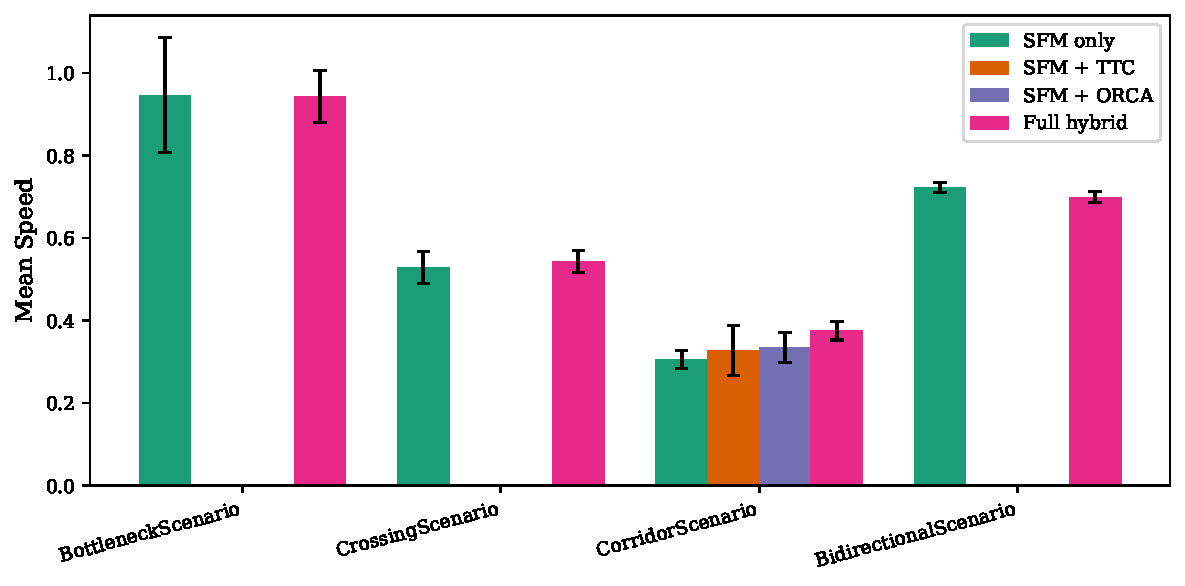
\includegraphics[width=\columnwidth]{../figures/ablation_mean_speed.pdf}
\caption{Mean speed by steering configuration (C1--C4) across bottleneck, bidirectional, and crossing scenarios ($n = 25$).}\label{fig:ablation}
\end{figure}

\subsection{Bottleneck Evacuation and Deadlock Resolution}
\label{sec:bottleneck-evac}

Table~\ref{tab:bottleneck} reports mean evacuation times ($n = 25$ replications) across five exit widths, with the C1 vs.\ C4 comparison tested using Welch's $t$-test.

\textbf{Normal exits (1.0--3.6\,m).}
At widths where evacuations complete normally, the hybrid produces a statistically significant evacuation-time reduction at narrow exits: 9.3\% at $w = 1.0$\,m ($p = 0.002$) and 7.4\% at $w = 1.2$\,m ($p < 0.001$).
At $w = 1.8$\,m, a 2.9\% reduction is marginally significant ($p = 0.045$).
At wide exits ($w \geq 2.4$\,m) the configurations converge to essentially identical evacuation times ($p > 0.1$) --- the expected asymptotic behaviour as congestion disappears (Figure~\ref{fig:evac_width}).

\textbf{Narrow exit deadlock ($w = 0.8$\,m).}
At a 0.8\,m exit with 100 agents and $n = 25$ replications, the four configurations reveal strikingly different deadlock-resolution capabilities:

\begin{center}
\scriptsize
\begin{tabular}{@{}lrrl@{}}
\toprule
\textbf{Config} & \textbf{Success} & \textbf{Rate} & \textbf{Interpretation} \\
\midrule
C1 (SFM) & 1/25 & 4\% & Stable arching \\
C2 (SFM+TTC) & 0/25 & 0\% & TTC worsens arching \\
C3 (SFM+ORCA) & 13/25 & 52\% & ORCA breaks arches \\
C4 (full hybrid) & 14/25 & 56\% & ORCA + TTC \\
\bottomrule
\end{tabular}
\end{center}

ORCA's velocity optimization is the mechanism that resolves the deadlock (C3: 52\%, C4: 56\%; Fisher's exact vs.\ C1: $p < 0.001$).
TTC alone does not help --- in fact C2 (0/25) performs \emph{worse} than C1 (1/25), suggesting that TTC's anticipatory deceleration reinforces rather than disrupts the symmetric force balance at the arch.
This decomposition --- TTC for collision reduction, ORCA for deadlock resolution --- is a key finding of the ablation.

\begin{table}[h]
\caption{Bottleneck evacuation time and collisions (mean$\pm$std, $n = 25$). $^{**}$\,$p < 0.01$; $^{*}$\,$p < 0.05$ (Welch C1 vs.\ C4 evacuation time). Collisions are nearly width-independent for $w \geq 1$\,m because most contacts occur during initial queue formation upstream of the exit (Section~\ref{sec:bottleneck-evac}).}\label{tab:bottleneck}
\centering
\scriptsize
\setlength{\tabcolsep}{3pt}
\begin{tabular}{@{}cllll@{}}
\toprule
\multicolumn{5}{l}{\textit{Evacuation time (s)}} \\
$w$\,(m) & \textbf{C1} & \textbf{C2} & \textbf{C3} & \textbf{C4} \\
\midrule
1.0 & 56.5$\pm$5.5 & 54.7$\pm$5.2 & 50.3$\pm$3.7 & \textbf{50.8$\pm$4.4}$^{**}$ \\
1.2 & 38.6$\pm$2.7 & 38.7$\pm$2.9 & 36.2$\pm$3.1 & \textbf{36.1$\pm$2.5}$^{**}$ \\
1.8 & 21.4$\pm$1.2 & 21.3$\pm$1.2 & 20.6$\pm$1.1 & \textbf{20.7$\pm$1.0}$^{*}$ \\
2.4 & 16.4$\pm$0.9 & 16.3$\pm$0.8 & 16.1$\pm$0.8 & \textbf{16.1$\pm$0.9} \\
3.6 & 13.0$\pm$0.7 & 13.1$\pm$0.8 & 12.6$\pm$0.7 & \textbf{12.8$\pm$0.7} \\
\midrule
\multicolumn{5}{l}{\textit{Collision count}} \\
$w$\,(m) & \textbf{C1} & \textbf{C2} & \textbf{C3} & \textbf{C4} \\
\midrule
1.0 & 42$\pm$17 & 30$\pm$12 & 41$\pm$15 & \textbf{29$\pm$12} \\
1.2 & 43$\pm$16 & 30$\pm$12 & 39$\pm$15 & \textbf{29$\pm$12} \\
1.8 & 42$\pm$16 & 30$\pm$12 & 39$\pm$15 & \textbf{29$\pm$12} \\
2.4 & 42$\pm$16 & 30$\pm$12 & 39$\pm$15 & \textbf{29$\pm$12} \\
3.6 & 42$\pm$16 & 30$\pm$12 & 39$\pm$15 & \textbf{29$\pm$12} \\
\bottomrule
\end{tabular}
\end{table}

\begin{figure}[!h]
\centering
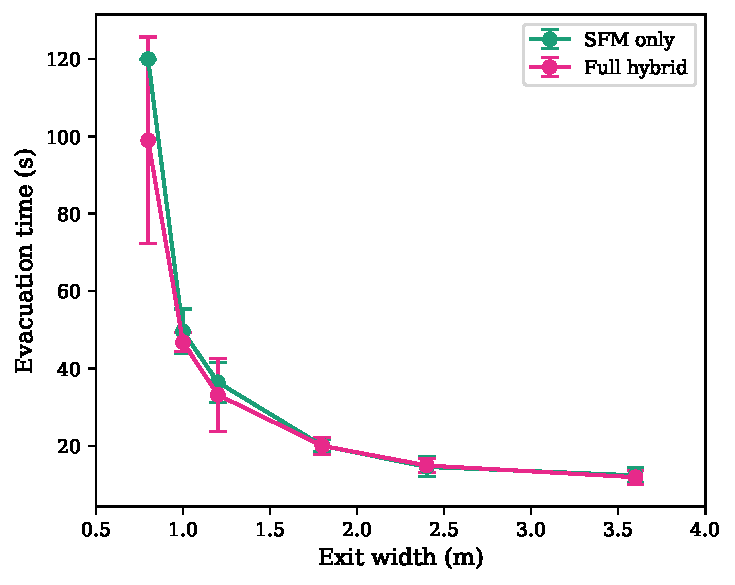
\includegraphics[width=\columnwidth]{../figures/evac_vs_width.pdf}
\caption{Evacuation time vs.\ exit width for C1 (SFM only) and C4 (full hybrid). Error bars: 95\% CIs, $n = 25$.}\label{fig:evac_width}
\end{figure}

\begin{figure}[!h]
\centering
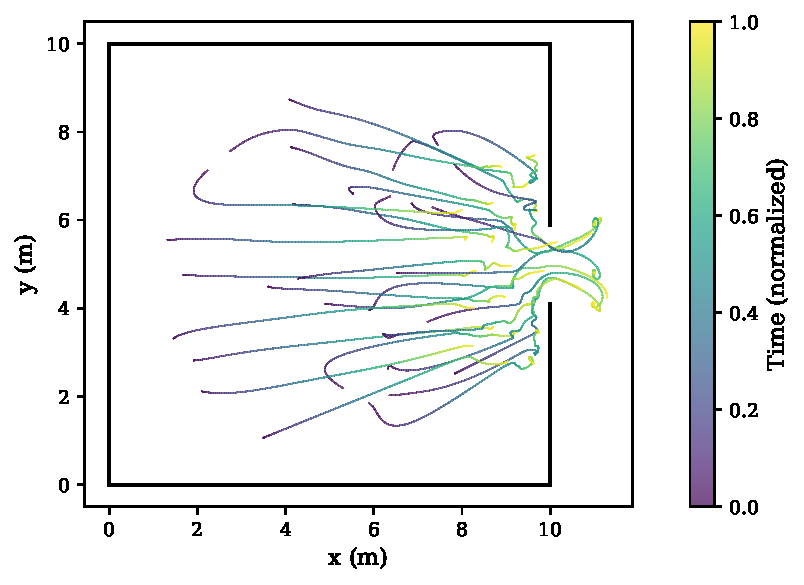
\includegraphics[width=\columnwidth]{../figures/trajectories.pdf}
\caption{Agent trajectories at the 0.8\,m bottleneck exit (100 agents, seed 46, same initial conditions). \textbf{Left:} C1 (SFM only) forms a stable arching deadlock at the exit; agents accumulate but cannot pass through within the 600\,s window. \textbf{Right:} C4 (full hybrid) destabilises the arch via ORCA's velocity-space optimisation and TTC's anticipatory evasion, evacuating all 100 agents in $\sim$134\,s. Colour: time progression (normalised). This pair illustrates the strongest qualitative result of the ablation: ORCA-enabled configurations resolve deadlocks that SFM alone cannot.}\label{fig:traj}
\end{figure}

\subsection{Computational Performance}
\label{sec:scaling-eval}

Figure~\ref{fig:scaling} shows per-step timing for C1 and C4 on a single CPU core (Python 3.11).
C1 rises from 2.9\,ms at 50 agents to 416\,ms at 1000 agents, following the sparse $O(N \cdot k)$ KDTree pair computation.
C4 is dominated by ORCA's per-agent LP: 131\,ms at 50 agents and 14{,}172\,ms at 500 agents (45--110$\times$ C1 overhead).
Real-time operation ($\leq$33\,ms/step) is achievable for C1 at $\sim$100 agents; C4 requires C/C++ acceleration of the ORCA loop.

\begin{figure}[!h]
\centering
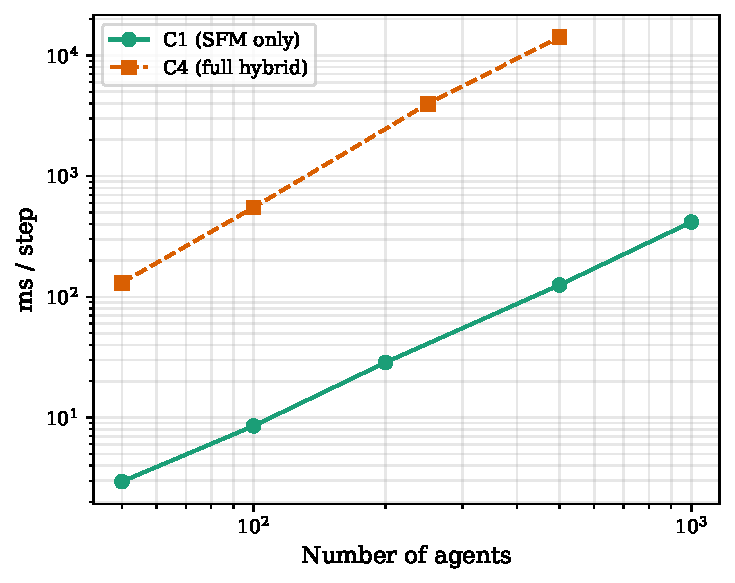
\includegraphics[width=0.85\columnwidth]{../figures/scaling.pdf}
\caption{Computation time per step vs.\ agent count (log-log). C1 (SFM only) and C4 (full hybrid). C4 overhead is dominated by ORCA's per-agent linear program ($\sim$45$\times$ slower than C1 at 50 agents).}\label{fig:scaling}
\end{figure}


%% ============================================================
%% SECTION 5: DISCUSSION
%% ============================================================
\section{\uppercase{Discussion}}
\label{sec:discussion}

\textbf{Why each steering component matters.}
The ablation reveals that TTC and ORCA serve \emph{distinct, complementary} roles rather than redundantly improving performance.
\textbf{TTC reduces collisions}: across all bottleneck widths, TTC-enabled configurations (C2, C4) consistently reduce collisions by 29--33\% relative to non-TTC configurations (C1, C3).
At 90\textdegree{} crossings, TTC's predictive evasion dissolves force-balance standoffs, tripling throughput.
\textbf{ORCA resolves deadlocks}: at the 0.8\,m exit, ORCA-enabled configurations (C3: 52\%, C4: 56\%) evacuate in roughly half of trials where SFM alone (C1: 4\%) and SFM+TTC (C2: 0\%) fail entirely.
The surprising finding that C2 performs \emph{worse} than C1 at deadlock resolution suggests that TTC's anticipatory deceleration reinforces the symmetric force balance at an arch, while ORCA's velocity-space optimisation breaks the symmetry by finding viable passage directions.

\textbf{Each component can be harmful in the wrong regime.}
The C2-worsens-deadlock finding has a mirror image: in bidirectional flow, ORCA alone (C3) reduces throughput from 68.9 to 63.9 exits because ORCA's collision-free velocity selection makes agents yield to counterflow neighbours, creating gridlock.
The full hybrid (C4: 73.7 exits) recovers throughput because TTC's collision reduction prevents the gridlock that pure ORCA yielding would cause.
Both negative results --- TTC harming deadlock resolution, ORCA harming counterflow throughput --- show that na\"ive always-on superposition of steering paradigms can be worse than any single paradigm.
This is precisely the motivation for the sigmoid-gated architecture: by weighting each component by local density, the framework activates each paradigm only in the regime where it helps and fades it out where it would hurt.

\textbf{Phenomenological calibration of the speed--density curve.}
Prior SFM-based studies report a ``calibration gap'' at mid-densities where textbook Weidmann parameters produce speeds above empirical data.
Our automated calibration (Section~\ref{sec:calibration}) treats this as a numerical fitting problem: a 4-parameter Nelder-Mead fit against binned FZJ data reduces the in-sample FD RMSE by 60.5\%.
This calibrates the desired-force speed--density relation only; because Figure~\ref{fig:fd} shows the FD is identical across C1--C4, this fit does \emph{not} validate the steering paradigm comparison and is reported as a phenomenological alignment of the speed--density curve.

\textbf{Limitations.}
Replication counts of $n = 25$ per cell reflect a fixed computational budget; effect sizes and per-condition sample sizes are reported throughout.
The 60\,s simulation windows for bidirectional and crossing measure steady-state throughput rather than total evacuation time, reflecting the computational cost of large-$N$ ORCA simulations.
The calibration is fit against FZJ unidirectional corridor data, so the 60.5\% RMSE reduction is an in-sample metric; held-out calibration against FZJ bottleneck trajectories is a natural next step.
% TODO R4: after R3.2 force-magnitude diagnostic, rewrite in past tense with actual crossover density.
The sigmoid threshold ($\rho_0 = 4.0$, slope $k = 2.0$) is motivated by the Fruin LoS-E boundary~\cite{Fruin71} and is not data-fitted; the force-magnitude diagnostic (Section~\ref{sec:experiments}) will provide empirical evidence for the crossover location.
The current sigmoid transitions are not hysteretic; we observed no oscillation artefacts in the present experiments but recommend hysteresis for deployments at densities sustained near $\rho_0$.


%% ============================================================
%% SECTION 6: CONCLUSIONS
%% ============================================================
\section{\uppercase{Conclusions}}
\label{sec:conclusion}

We presented a diagnostic ablation of three pedestrian steering paradigms --- SFM, TTC, and ORCA --- that identifies two failure modes single-paradigm models cannot avoid: TTC anticipation locks symmetric arches at narrow exits (0/25 versus 1/25 for plain SFM), and ORCA-style yielding produces gridlock in counterflow. A density-adaptive convex combination of the three paradigms mitigates each failure mode, resolving arching deadlocks in 56\% of trials versus 4\% for SFM alone (Fisher's exact $p < 0.001$) and tripling throughput at 90\textdegree{} crossings ($p < 0.001$). The Weidmann speed--density curve was calibrated phenomenologically against 4776 FZJ data points (in-sample RMSE reduction 60.5\%), but because the FD is identical across C1--C4 this calibration validates only the desired-force speed reduction and not the steering paradigms themselves. Code, data, and reproduction scripts are released with the paper.

Future work targets held-out calibration on FZJ bottleneck trajectories, C/C++ acceleration of the ORCA linear program, and integration into digital twin pipelines for real-time venue monitoring.

%% ============================================================
%% REFERENCES
%% ============================================================

\bibliographystyle{apalike}
{\small
\bibliography{references}}

\end{document}
